\documentclass{article}

\usepackage{fancyhdr}
\usepackage{extramarks}
\usepackage{amsmath}
\usepackage{amsthm}
\usepackage{amsfonts}
\usepackage{amssymb}
\usepackage{xparse}
\usepackage{tikz}
\usepackage{graphicx}
\usepackage[plain]{algorithm}
\usepackage{algpseudocode}
\usepackage{listings}
\usepackage{hyperref}
\usepackage[per-mode = fraction]{siunitx}
\usepackage{calc}

\usetikzlibrary{automata,positioning}

\hypersetup{
    colorlinks=true,
    linkcolor=blue,
    filecolor=magenta,
    urlcolor=blue,
    }

\urlstyle{same}

%
% Basic Document Settings
%

\topmargin=-0.45in
\evensidemargin=0in
\oddsidemargin=0in
\textwidth=6.5in
\textheight=9.0in
\headsep=0.25in

\linespread{1.1}

\pagestyle{fancy}
\lhead{\hmwkAuthorName}
\chead{\hmwkClass\ (\hmwkClassInstructor,\ \hmwkClassTime): \hmwkTitle}
\rhead{\firstxmark}
\lfoot{\lastxmark}
\cfoot{\thepage}

\renewcommand\headrulewidth{0.4pt}
\renewcommand\footrulewidth{0.4pt}

\setlength\parindent{0pt}
\allowdisplaybreaks
%
% Title Page
%

\title{
	\vspace{2in}
	\textmd{\textbf{\hmwkClass:\ \hmwkTitle}}\\
	\normalsize\vspace{0.1in}\small{Due\ on\ \hmwkDueDate\ at \hmwkDueTime}\\
	\vspace{0.1in}\large{\textit{\hmwkClassInstructor,\ \hmwkClassTime}}
	\vspace{3in}
}
\author{\textbf{\hmwkAuthorName}}
\date{\hmwkCompletionDate}

%
% Create Problem Sections
%

\newcommand{\enterProblemHeader}[1]{
	\nobreak\extramarks{}{Problem #1 continued on next page\ldots}\nobreak{}
	\nobreak\extramarks{Problem #1 (continued)}{Problem #1 continued on next page\ldots}\nobreak{}
}

\newcommand{\exitProblemHeader}[1]{
	\nobreak\extramarks{Problem #1 (continued)}{Problem #1 continued on next page\ldots}\nobreak{}
	\nobreak\extramarks{Problem #1}{}\nobreak{}
}

%
% Homework Problem Environment
%
\NewDocumentEnvironment{hwkProblem}{m m s}{
	\section*{Problem #1: #2}
	\enterProblemHeader{#1}
	\setcounter{partCounter}{1}
}{
	\exitProblemHeader{#1}
	\IfBooleanF{#3} % if star, no new page
		{\newpage}
}

% Alias for the Solution section header
\newcommand{\hwkSol}{\vspace{\baselineskip / 2}\textbf{\Large Solution}\vspace{\baselineskip / 2}}

% Alias for the Solution Part subsection header
\newcounter{partCounter}
\newcommand{\hwkPart}{
	\vspace{\baselineskip / 2}
	\textbf{\large Part \Alph{partCounter}}
	\vspace{\baselineskip / 2}
	\stepcounter{partCounter}
}

%
% Various Helper Commands
%

% Such That
\newcommand{\st}{\text{s.t.}}

% Useful for algorithms
\newcommand{\alg}[1]{\textsc{\bfseries \footnotesize #1}}

% For derivatives
\newcommand{\deriv}[1]{\frac{\mathrm{d}}{\mathrm{d}x} (#1)}

% For partial derivatives
\newcommand{\pderiv}[2]{\frac{\partial}{\partial #1} (#2)}

% Integral dx
\newcommand{\dx}{\mathrm{d}x}
\newcommand{\dy}{\mathrm{d}y}

% Probability commands: Expectation, Variance, Covariance, Bias
\newcommand{\e}[1]{\mathrm{e}#1}
\newcommand{\E}{\mathrm{E}}
\newcommand{\Var}{\mathrm{Var}}
\newcommand{\Cov}{\mathrm{Cov}}
\newcommand{\Bias}{\mathrm{Bias}}

% Defining Units that are not in the SI base
\DeclareSIUnit\bar{bar}
\DeclareSIUnit\ft{ft}
\DeclareSIUnit\dollar{\$}
\DeclareSIUnit\cent{\text{\textcent}}
\DeclareSIUnit\c{\degreeCelsius}

% Code Listing config
\usepackage{xcolor}
\definecolor{codegreen}{rgb}{0,0.6,0}
\definecolor{codegray}{rgb}{0.5,0.5,0.5}
\definecolor{codepurple}{rgb}{0.58,0,0.82}
\definecolor{backcolour}{rgb}{0.95,0.95,0.92}
\lstdefinestyle{overleaf}{
	% backgroundcolor=\color{backcolour},
	commentstyle=\color{codegreen},
	keywordstyle=\color{magenta},
	numberstyle=\tiny\color{codegray},
	stringstyle=\color{codepurple},
	basicstyle=\ttfamily\footnotesize,
	breakatwhitespace=false,
	breaklines=true,
	captionpos=b,
	keepspaces=true,
	numbers=left,
	numbersep=5pt,
	showspaces=false,
	showstringspaces=false,
	showtabs=false,
	tabsize=4
}

\usepackage[latte]{catppuccinpalette}
\lstdefinestyle{catppuccin}{
	breaklines=true,
	keepspaces=true,
	numbers=left,
	numbersep=5pt,
	showspaces=false,
	showstringspaces=false,
	breakatwhitespace=true,
	tabsize=4,
	stringstyle = {\color{CtpGreen}},
	commentstyle={\color{CtpOverlay1}},
	basicstyle = {\small\color{CtpText}\ttfamily},
	keywordstyle = {\color{CtpMauve}},
	keywordstyle = [2]{\color{CtpBlue}},
	keywordstyle = [3]{\color{CtpYellow}},
	keywordstyle = [4]{\color{CtpLavender}},
	keywordstyle = [5]{\color{CtpPeach}},
	keywordstyle = [6]{\color{CtpTeal}}
}

\lstset{style=catppuccin}


%
% Homework Details
%   - Title
%   - Due date
%   - Class
%   - Section/Time
%   - Instructor
%   - Author
%

\newcommand{\hmwkTitle}{Week 01 Discussion}
\newcommand{\hmwkDueDate}{September 02, 2024}
\newcommand{\hmwkDueTime}{11:59 PM}
\newcommand{\hmwkClass}{HISP 200}
\newcommand{\hmwkClassTime}{Section 0101}
\newcommand{\hmwkClassInstructor}{Prof. Woehlke}
\newcommand{\hmwkAuthorName}{\textbf{Vai Srivastava}}

\begin{document}

\maketitle

\pagebreak

\begin{homeworkProblem}

	Draw a map from memory of the landscape or environment that you have a personal connection to.
	\begin{enumerate}
		\item Include buildings, paths, vegetation/plantings, etc.
		\item Label structures, roads, businesses, etc.
		\item Are there additional elements that contribute to the cultural significance, meaning, and memory of this place, like statues, murals, signage, languages represented, etc.?
	\end{enumerate}

	\solution

	\begin{figure}[h]
		\begin{center}
			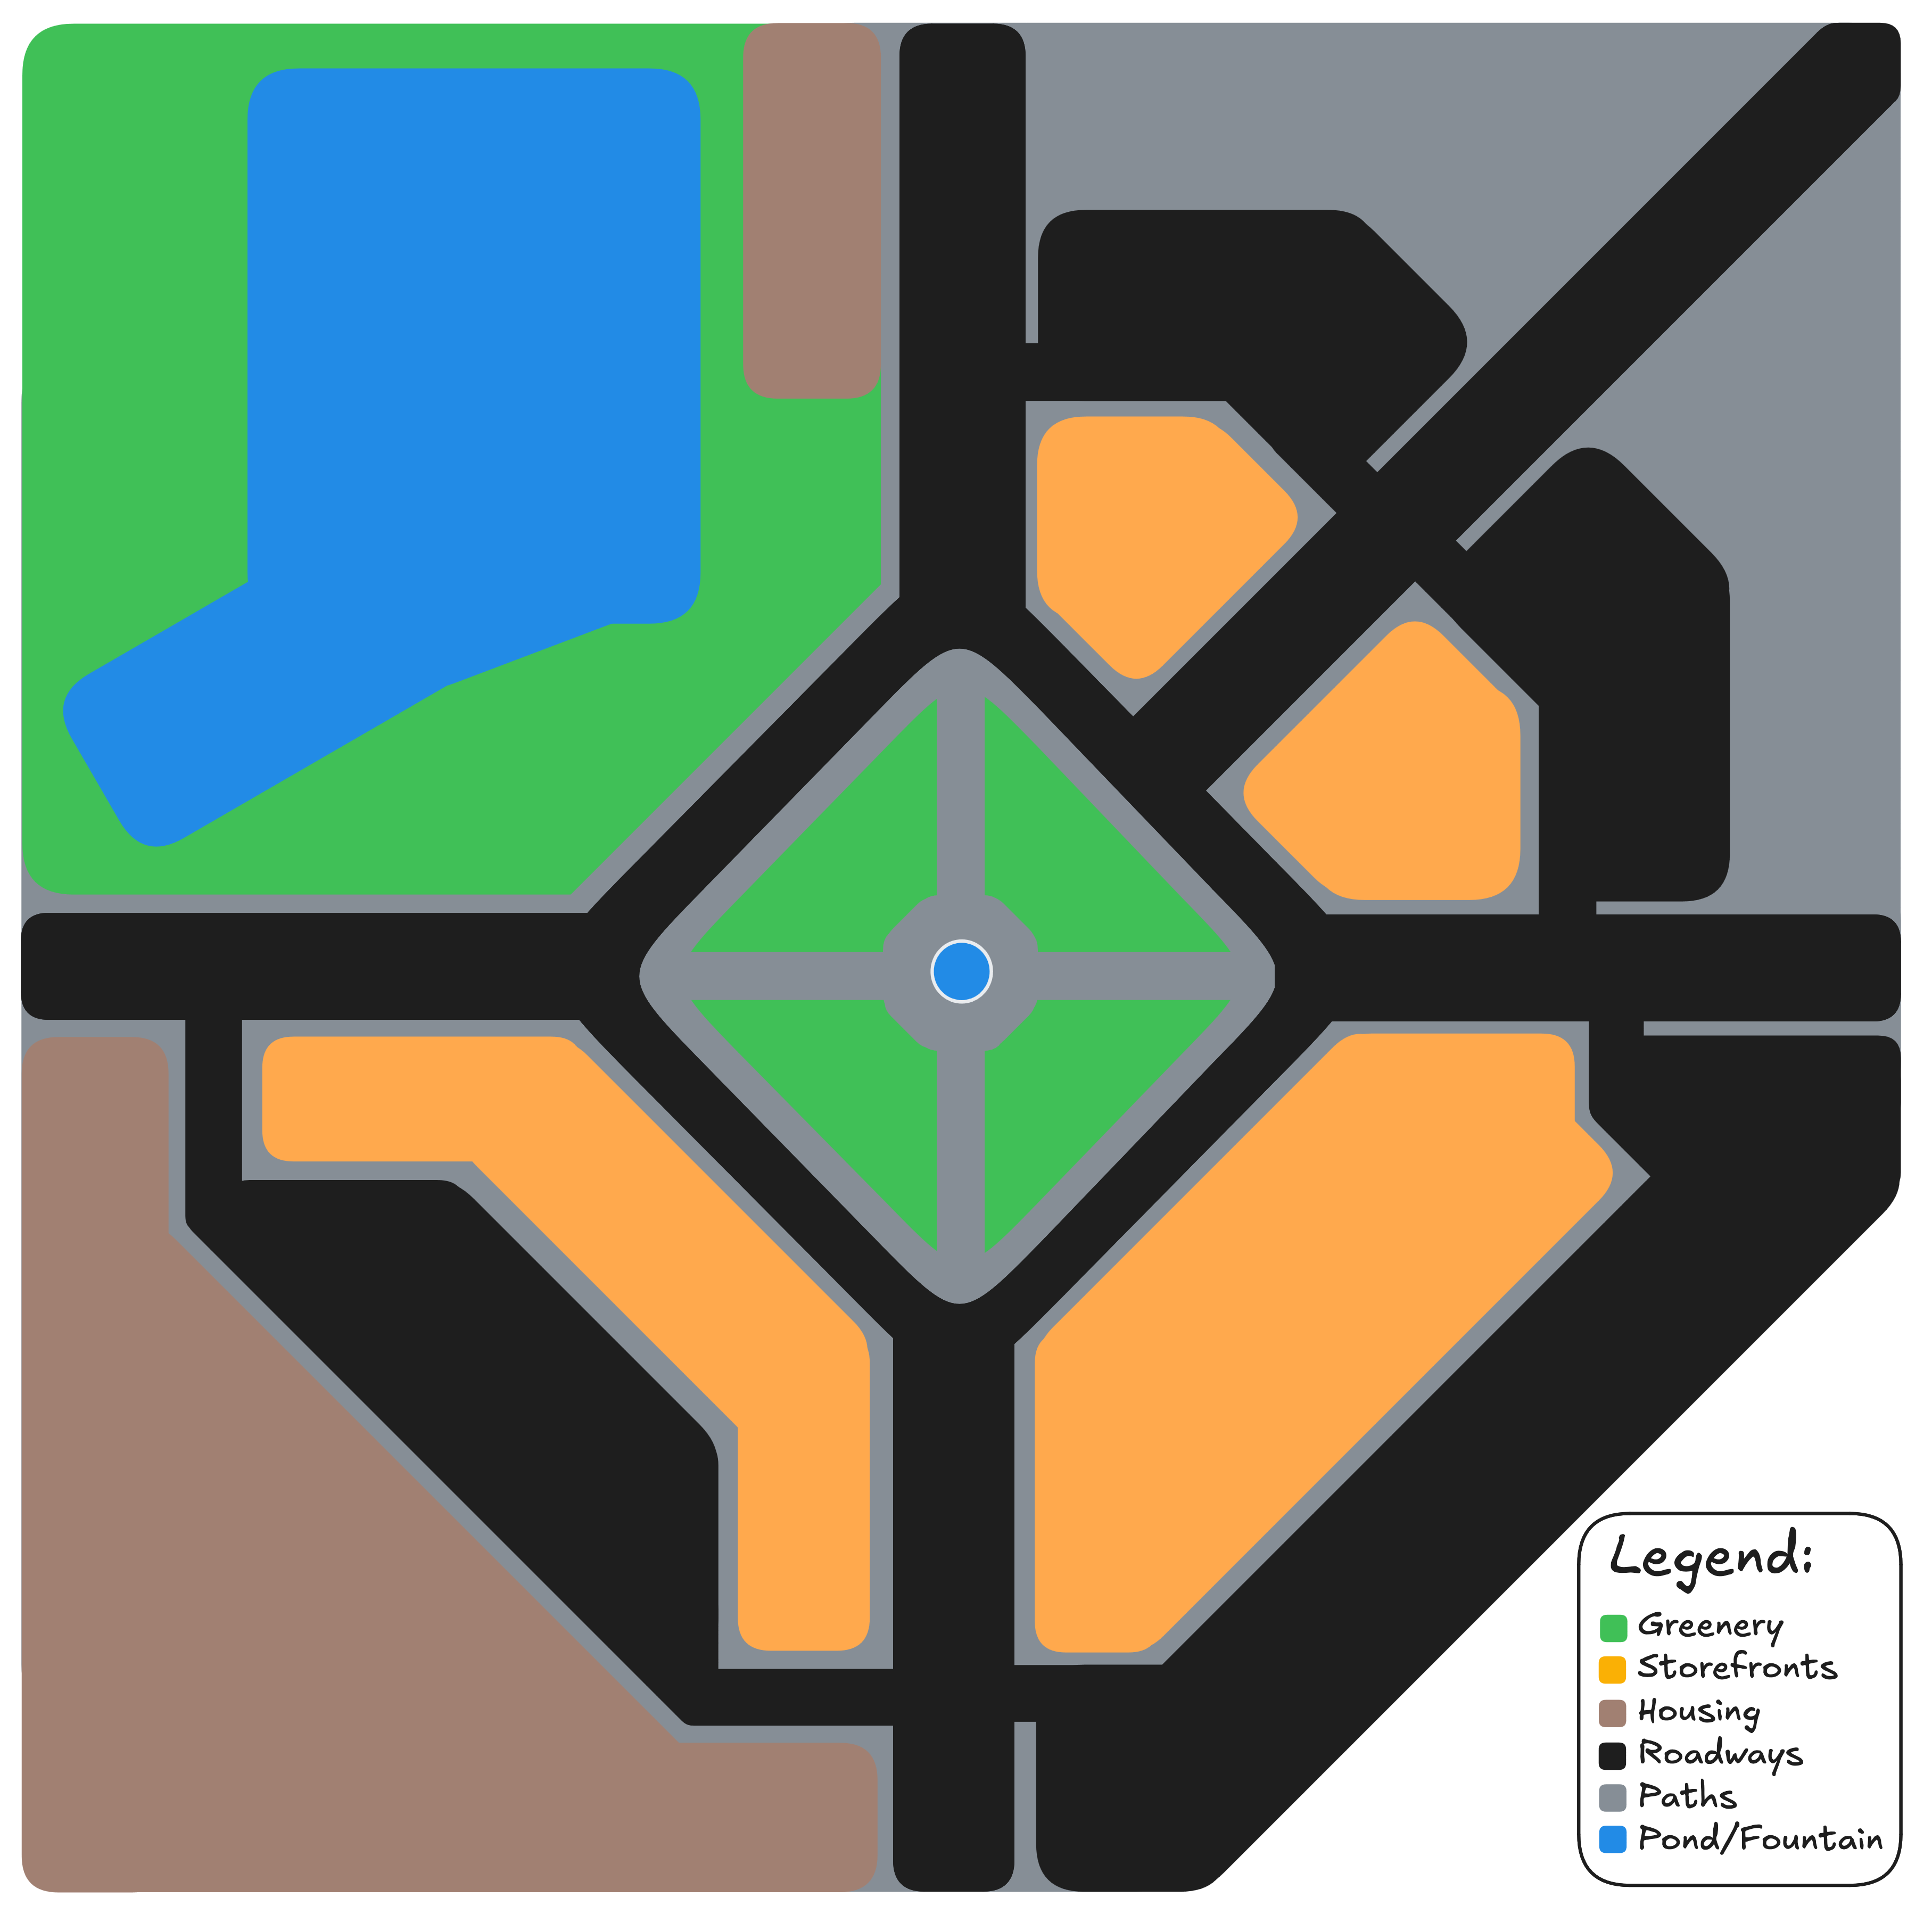
\includegraphics[width=0.65\textwidth]{images/map.png}
		\end{center}
		\caption{Map of Evergreen Village Square in San Jose, California}\label{fig:w01 map}
	\end{figure}


\end{homeworkProblem}

\begin{homeworkProblem}

	What do you think are some of the intentions of the designers of this space?

	\solution

	I believe the designers of this space intended for people to be able to walk around and across the square, as foot traffic in the middle of a neighborhood is quite important. As well, the designers intentionally kept the roadways narrow, with angled parking spaces, in order to increase pedestrian safety and encourage slower driving and pedestrian safety.

\end{homeworkProblem}

\begin{homeworkProblem}

	How do people respond to this intent?

	\solution

	People use the space as intended, with drivers going quite slowly, and many pedestrians frequenting the center park. The layout of the Village Square, with paths cutting through the park in the center, and a large walkway all the way around lends well to markets popping up, and as such, there is a farmer's market every Wednesday and Sunday.

\end{homeworkProblem}

\begin{homeworkProblem}

	Do you believe people are aware of the designers' intentions, or not? Why?

	\solution

	I do not believe that people are aware of the designers' intentions. For one, many of the people in the area are children, due to the Village Square's proximity to neighborhoods and multiple schools. As well, I have heard many drivers begrudge the thin roads, complaining about having to slow down when passing through the area.

\end{homeworkProblem}

\begin{homeworkProblem}

	Does the design influence the way the place is used by people?

	\solution

	Yes, most definitely. The design of the area has contributed to the local economy and businesses, while also providing a safe third-space for children to socialize after school.

\end{homeworkProblem}

\begin{homeworkProblem}

	In what ways is this built environment used that are outside of the designers' expectation?

	\solution

	This built environment is used for parties and large childrens' games (like toy gun battles and water tag), which is likely outside of the designers' expectations. Many of the design elements of the Village Square are directly geared towards traffic and flow through the area, as well as accomodating those who wish to conduct business or enjoy a calm evening there. These games, which often rely on hiding behind benches, trees, bushes, and even cars, were likely not in mind when the designers were planning the space.

\end{homeworkProblem}
\end{document}
